% use paper, or submit
% use 11 pt (preferred), 12 pt, or 10 pt only

\documentclass[letterpaper, preprint, paper,11pt]{AAS}	% for preprint proceedings
%\documentclass[letterpaper, paper,11pt]{AAS}		% for final proceedings (20-page limit)
%\documentclass[letterpaper, paper,12pt]{AAS}		% for final proceedings (20-page limit)
%\documentclass[letterpaper, paper,10pt]{AAS}		% for final proceedings (20-page limit)
%\documentclass[letterpaper, submit]{AAS}			% to submit to JAS

\usepackage{bm}
\usepackage{amsmath}
\usepackage{subfigure}
%\usepackage[notref,notcite]{showkeys}  % use this to temporarily show labels
\usepackage[colorlinks=true, pdfstartview=FitV, linkcolor=black, citecolor= black, urlcolor= black]{hyperref}
\usepackage{overcite}
\usepackage{footnpag}			      	% make footnote symbols restart on each page


% added by Sara
\usepackage{enumitem} % for bullet points
%\usepackage{graphicx} % for displaying images
\graphicspath{ {./Figures/} } % search path for images
\usepackage{booktabs} % for making tables in professional style with top and bottom border
\usepackage{textcomp} % for degree symbol
%\usepackage{fullpage} % for reducing page margins
%\usepackage{float}    % to keep figures with text
%\usepackage{afterpage} % used with \afterpage{\clearpage}... not sure if it's doing anything helpful




\PaperNumber{15-747}


\begin{document}

\title{Libration Point Orbit Rendezvous Using Linearized Relative Motion Dynamics and Nonlinear Differential Correction}

\author{Sara Case\thanks{Department of Aerospace Engineering, University of Maryland, College Park}}

\maketitle{} 		

\begin{abstract}
This paper presents a technique for computing a rendezvous trajectory with a target satellite in a libration point orbit.  The chaser satellite completes the rendezvous by executing a series of impulsive maneuvers to travel between waypoints approaching the target satellite.  Linearized equations of relative motion of the chaser with respect to the target in the circular restricted three body problem are used to compute the required magnitude and direction of the maneuvers; these results are then refined using differential correction with the nonlinear equations of motion. The performance of this technique is discussed and several rendezvous strategies are evaluated.
\end{abstract}

\section{Introduction}
Libration point orbit rendezvous is a critical component for many possible satellite mission architectures.  If a large satellite is launched in components and assembled in orbit, the individual components will need to rendezvous and dock prior to assembly.  If a valuable space asset such as a telescope requires an on-orbit repair, the satellite servicing mission will need to rendezvous with the object.  A libration point orbit is a potentially useful place to build a space station, and rendezvous capabilities will be important during the construction of the station as well as every crew and cargo mission to visit the station.

The history of satellites being deployed to libration point orbits dates back to 1978, when ISEE-3 was launched to the Sun-Earth L1 point. ACE, WIND, SOHO, and DSCOVR are currently orbiting the same point, with the LISA Pathfinder satellite set to join them in 2015.  Several spacecraft have been deployed to the Sun-Earth L2 point, and the ARTEMIS mission explored L1 and L2 in the Earth-Moon system.  Several additional libration point orbiting missions are currently planned, including the James Webb Space Telescope.  So far, all libration point missions have consisted of a single satellite that operates independently of any other satellite.  There has been research on deploying a formation of satellites to fly together around libration points, such as the Terrestrial Planet Finder mission.\cite{beichman2004}  However, little research has been conducted regarding rendezvous with libration point orbiters. % TODO: (refer to a paper about building a space station at a libration point)

Satellite rendezvous in low-Earth orbit is well-studied, due to many years of experience operating the International Space Station and other applications.  The Hill's/Clohessy-Wiltshire (HCW) equations are frequently used to closely approximate the relative motion of a chaser vehicle with respect to a target vehicle in a circular orbit.\cite{clohessy1960}  These equations of relative motion are used to compute the approximate \(\Delta V\) (instantaneous change in velocity) to travel between waypoints defining an approach trajectory.  However, for libration point orbits, the dynamical environment is quite different and the same equations of motion are not applicable.  % TODO: (cite rendezvous ISS paper) (mention r-bar, v-bar?)

Luquette has developed linearized equations of relative motion for formation flying in libration point orbits.\cite{luquette2004}   Lian et al.~have used these linearized dynamics to compute impulses for a chaser satellite to travel between waypoints in order to approach a target orbiting a libration point.\cite{lian2011}  This paper discusses the results of applying this technique for a set of test cases, and presents an additional step in which the shooting method of differential correction is used to refine the computed \(\Delta V\) for use with the nonlinear equations of motion.  % "set of test cases in the Earth-Moon L1 system"

\section{Dynamics}

\subsection{Circular Restricted Three-Body Dynamics}
The circular restricted three body problem (CRTBP) deals with two larger objects orbiting each other in a circular orbit and a third object of infinitesimal mass.  Examples include the Trojan asteroids orbiting in the Sun-Jupiter system, or man-made satellites in the Earth-Moon system.  When dealing with the Sun-Earth system, the second body is often modeled by treating the Earth and Moon as a single object at the Earth-Moon barycenter; this is called the Sun-Earth/Moon system.

The nonlinear equations of motion for a satellite in the CRTBP are:

\begin{equation} \label{eq:CRTBP}
	\begin{aligned}
		\ddot{x} &= x + 2\dot{y} + \frac{(1 - \mu)(-\mu - x)}{r_1^3} + \frac{\mu(1 - \mu - x)}{r_2^3} \\
		\ddot{y} &= y - 2\dot{x} - \frac{(1 - \mu)y}{r_1^3} - \frac{\mu y}{r_2^3} \\
		\ddot{z} &= \frac{-(1 - \mu)z}{r_1^3} - \frac{\mu z}{r_2^3}
	\end{aligned}
\end{equation}

where \(\mu\) is the mass ratio of the primary bodies:

\begin{equation}
	\mu = \frac{M_2}{M_1 + M_2}
\end{equation}

and \(r_1\) and \(r_2\) are the distances from the larger and smaller bodies to the target satellite:

\begin{equation}
	\begin{aligned}
		r_1 &= \| \mathbf{x} - \mathbf{X_1} \| &= \sqrt{(x-\mathbf{X_1}_x)^2 + y^2 + z^2} \\
		r_2 &= \| \mathbf{x} - \mathbf{X_2} \| &= \sqrt{(x-\mathbf{X_2}_x)^2 + y^2 + z^2}
	\end{aligned}
\end{equation}

where \(\mathbf{X_1}\) and \(\mathbf{X_2}\) are the positions of the larger and smaller bodies along the X-axis of the rotating CRTBP frame:

\begin{equation}
	\begin{aligned}
		\mathbf{X_1} &= \begin{bmatrix}
			-\mu \\ 0 \\ 0 
		\end{bmatrix} \\
		\mathbf{X_2} &= \begin{bmatrix}
			1 - \mu \\ 0 \\ 0
		\end{bmatrix}
	\end{aligned}
\end{equation}

When working in canonical units in the CRTBP, one distance unit is defined by the distance between the primary bodies, one mass unit is defined by the combined mass of the primary bodies, and one time unit is defined by the period of the primary bodies divided by 2\(\pi\).  Finally, the gravitational constant G is also defined as one. Note that as a result, the rotation rate of the system \(\omega\) also evaluates to one. A summary of the canonical units in the CRTBP is provided in Equation~\eqref{eq:nondimen}.

\begin{equation} \label{eq:nondimen}
\begin{aligned}
\mathrm{1 \: DU} &= r_{12} = 1 \\           % note, "\:" is a medium space
\mathrm{1 \: MU} &= M_1 + M_2 = 1 \\
\mathrm{1 \: TU} &= \frac{P}{2\pi} = 1 \\
\mathrm{G} &= 1 \\
\omega &= \sqrt{GM/r^3} = 1
\end{aligned}
\end{equation}

\subsection{Linearized Relative Motion Dynamics}
Luquette has derived linearized equations of relative motion of a chaser satellite with respect to a target satellite orbiting in the restricted three body problem (RTBP).\cite{luquette2004} The RTBP is distinct from the CRTBP discussed above in that the RTBP provides the option to model the primary bodies in an elliptic orbit instead of a circular orbit around each other; the rotation rate of the system is therefore a function of time. Luquette provides the equations of relative motion in two reference frames: the inertial frame as well as the rotating (RTBP) frame.  These equations of motion are valid anywhere in the RTBP system; they are not assumed to be near any specific libration point.  They are also useful for analyzing relative motion around any type of libration point orbit, such as Lyapunov, halo, or Lissajous orbits. 

In this work, the equations of motion as given in the rotating reference frame are used. These equations are functions of the offset state of the chaser vehicle with respect to the target vehicle in the rotating frame, the position of the target vehicle in the rotating frame with respect to the origin, the mass ratio of the primary bodies, and the rotation rate of the rotating frame.

% TODO: Should I also include the inertial version of the relmo EOM's from Luquette?  I only used the rotating frame version, but maybe the inertial version should also be provided for completeness.  Could simply say that the inertial version doesn't have the \(\omega\) terms and all the vectors are in the inertial frame instead of CRTBP.

The linearized equations of relative motion of a chaser satellite with respect to a target satellite, given in the RTBP reference frame, are:

\begin{equation} \label{eq:RelmoDerivs}
	\dot{\boldsymbol{\xi}}_R = \mathbf{A}_R(t)\boldsymbol{\xi}_R
\end{equation}

where \(\boldsymbol{\xi}_R\) is the offset state of the chaser vehicle with respect to the target vehicle in the rotating frame:

\begin{equation}  % Note, R is for "rotating" and C is for "chaser"
	\boldsymbol{\xi}_R = \begin{bmatrix}
		\mathbf{x}_c \\
		\dot{\mathbf{x}}_c
	\end{bmatrix}_R
\end{equation}

and  \(\mathbf{A}_R(t)\) is the 6\(\times\)6 linearized relative motion dynamics matrix in the rotating frame: % note, in the paper I'm citing, he says \(-2 [\boldsymbol{\omega} \times]^T\), but in his PhD it just says \(-2 [\boldsymbol{\omega} \times]\) which seems to be correct

\begin{equation} \label{eq:RelmoDynMatrix}
	\mathbf{A}_R(t) = \begin{bmatrix}
		\mathbf{0}          & \mathbf{I_3} \\
		\mathbf{\Xi}_R(t) & -2 [\boldsymbol{\omega} \times]
	\end{bmatrix}
\end{equation}

where

\begin{equation}
	\mathbf{\Xi}_R(t) = -(c_1 + c_2)\mathbf{I_3} 
	+ 3c_1\mathbf{\hat{r}_1}(t) \mathbf{\hat{r}_1}(t)^T 
	+ 3c_2\mathbf{\hat{r}_2}(t) \mathbf{\hat{r}_2}(t)^T 
	+ [\boldsymbol{\dot{\omega}} \times] 
	- [\boldsymbol{\omega}\times][\boldsymbol{\omega}\times]
\end{equation}

and

\begin{equation}
	\begin{aligned}
		c_1 &= \frac{1- \mu}{r_1^3} \\
		c_2 &= \frac{\mu}{r_2^3}
	\end{aligned}
\end{equation}

Note that \(\boldsymbol{\omega}\) is the rotation rate of the rotating RTBP frame with respect to the inertial frame:
\begin{equation}
	\boldsymbol{\omega} = \begin{bmatrix}
		0 \\ 
		0 \\
		\omega
	\end{bmatrix}
\end{equation}

The notation  \([\boldsymbol{\omega}\times]\) refers to the cross-product matrix of \(\boldsymbol{\omega}\):
\begin{equation}
	[\boldsymbol{\omega}\times] = \begin{bmatrix}
		0           & -\omega & 0 \\ 
		\omega & 0             & 0 \\
		0           & 0             & 0
	\end{bmatrix}
\end{equation}

Also note that if we assume that the rotation rate of the RTBP frame is constant (that is, assume we can use the CRTBP where the massive bodies are in circular orbits around each other), then the \(\boldsymbol{\dot{\omega}}\) term cancels to zero.

These equations of motion do not include any model of solar radiation pressure (SRP) and assume that neither satellite is applying any propulsive thrusting force to perturb or change their orbits. 

In order to integrate a chaser satellite's trajectory using the equations of relative motion given in Equation~\eqref{eq:RelmoDerivs}, the integration state vector must contain the absolute state of the target satellite in the RTBP frame (with respect to the origin of the RTBP frame) and the relative state of the chaser satellite in the RTBP frame (with the origin located at the target satellite).  If using the CRTBP assumption, then the target satellite's state over time can be integrated using the classical CRTBP equations of motion as given in Equation~\eqref{eq:CRTBP}, which must be done concurrently with the integration of the relative motion of the chaser so that the time-dependent linearized relative motion dynamics matrix \(\mathbf{A}_R(t)\) given in Equation~\eqref{eq:RelmoDynMatrix} can be computed. The CRTBP model is employed in the test cases presented in this work.

\section{Traveling Between Waypoints with Impulsive $\Delta$V's}
The concept of waypoints can be used to divide a rendezvous approach trajectory into a series of shorter segments.  The starting and ending waypoints of a segment are defined with respect to the location of a target satellite.  When considering rendezvous with a satellite in a circular orbit, the HCW equations supply a linearized dynamics model for a chaser satellite with respect to a target satellite.  The inverse of the linear dynamics matrix is used to compute the velocity required to travel from one waypoint to the next within a specified amount of time.  This approach is applied in the CRTBP using the linear dynamics matrix presented in Equation~\eqref{eq:RelmoDynMatrix} by following the procedure below. 

\subsection{Using the Linearized Relative Motion Dynamics Matrix to Compute \(\Delta\)V}

The linearized relative motion dynamics matrix given in Equation~\eqref{eq:RelmoDynMatrix} can be used to numerically accumulate a State Transition Matrix (STM), \(\boldsymbol{\Phi}\), of the chaser satellite with respect to the target satellite over time:

\begin{equation} \label{eq:STM}
	\dot{\boldsymbol{\Phi}} = \mathbf{A}_R(t)\boldsymbol{\Phi}
\end{equation}

The initial ``state vector" for the STM passed to the integration process should be the \(6\times6\) identity matrix, \(\mathbf{I_6}\).  As above, the STM must be integrated concurrently with the target satellite's state because of the time-dependence in \(\mathbf{A}_R(t)\).  When integrated from the initial state at time \(t_i\) to a future time \(t_{i+1}\), this accumulated State Transition Matrix represents the relative position and velocity of the chaser at time \(t_{i+1}\) with respect to its relative position and velocity at time \(t_i\).  More explicitly:

% TODO!!!: need to make notation consistent; should it be r, v or x, xdot, or xi, xidot, or what

\begin{equation}
	\begin{bmatrix}
		\mathbf{r}_{i+1} \\
		\mathbf{v}_{i+1}
	\end{bmatrix}
	= 
	\begin{bmatrix}
		\boldsymbol{\Phi}_{11} & \boldsymbol{\Phi}_{12} \\
		\boldsymbol{\Phi}_{21} & \boldsymbol{\Phi}_{22}
	\end{bmatrix}
	\begin{bmatrix}
		\mathbf{r}_i \\
		\mathbf{v}_i
	\end{bmatrix}
\end{equation}

Analogous to the use of the HCW equations in the two-body problem, this STM can be used to compute the required velocity \(\mathbf{v}_i^+\) for a chaser satellite in a CRTBP system to travel from waypoint \(\mathbf{r}_i\) to waypoint \(\mathbf{r}_{i+1}\) in time \( \Delta t = t_{i+1} - t_i\).  This approach was employed by Lian et al.~using the RTBP relative motion dynamics derived by Luquette (see Reference \citenum{lian2011}). 

% TODO: maybe note: Lian et. al. used the equations with J2000 reference axes and equations of motion written in J2000, rather than the rotating frame (RTBP) version being used here.

% TODO: cite additional Lian papers.

\begin{equation} \label{eq:RequiredVelocity}
	\mathbf{v}_i^+ = \boldsymbol{\Phi}_{12}^{-1}(\mathbf{r}_{i+1} - \boldsymbol{\Phi}_{11}\mathbf{r}_i)
\end{equation}

The instantaneous change in velocity (\(\Delta V\)) for a maneuver at waypoint \(\mathbf{r}_i\) is then simply the difference between the required (post-maneuver) velocity and the velocity that the chaser satellite had before the maneuver:

\begin{equation} \label{eq:DeltaV}
	\Delta \mathbf{v}_i = \mathbf{v}_i^+ - \mathbf{v}_i^-
\end{equation}

\subsection{Shooting Method with Nonlinear Dynamics} \label{sec:shooting}
The approach described above for computing \(\Delta V\) is based on the linearized equations of relative motion developed by Luquette.  Of course, the true dynamical environment in the CRTBP is nonlinear, as seen in Equation~\eqref{eq:CRTBP}. The linear-based approximation of \(\Delta V\) can be corrected for use with this nonlinear propagation model using the shooting method of differential correction.  The linear-based approximated velocity is used as an initial guess for this iterative process.  Following the procedure below, each of the three components of the velocity vector is varied in order to achieve convergence in the CRTBP on the desired three-dimensional waypoint \(\mathbf{w}_{\mathrm{desired}}\) within some specified tolerance.

\begin{enumerate}[leftmargin=!,labelindent=12pt,itemindent=0pt, label=Step \arabic*:]
	
	\item Using the initial guess for the chaser relative velocity \(\mathbf{v}_i^+\) from Equation~\eqref{eq:RequiredVelocity}, propagate both the target and chaser satellite from time \(t_i\) to \(t_{i+1}\) using the nonlinear CRTBP equations of motion given in Equation~\eqref{eq:CRTBP} and compute the nominally achieved waypoint \(\mathbf{w}\).
	
	\item Add to the x-component of the chaser's velocity a pre-chosen scalar value, called the perturbation.  Propagate both satellites from time \(t_i\) to \(t_{i+1}\) a second time using this perturbed velocity and compute the achieved waypoint \(\mathbf{w}'\).
	
	\item Compute the difference between \(\mathbf{w}\) and \(\mathbf{w}'\), \(\frac{d\mathbf{w}}{dv_x}\).
	
	\item Reset the x-component of the velocity to its original value, and repeat steps 2 and 3 when perturbing the y-component of the velocity.
	
	\item Reset the y-component of the velocity to its original value, and repeat steps 2 and 3 when perturbing the z-component of the velocity.
	
	\item Gather the results into a partial derivatives matrix, \(\mathbf{M}\):
	
	\begin{equation} \label{eq:ShootingMethodPartialDerivs}
		\mathbf{M} = \left[ \frac{d\mathbf{w}}{d\mathbf{v}} \right]
		= \begin{bmatrix}
			\frac{dw_x}{dv_x} & \frac{dw_y}{dv_x} & \frac{dw_z}{dv_x} \\[0.3em]
			\frac{dw_x}{dv_y} & \frac{dw_y}{dv_y} & \frac{dw_z}{dv_y} \\[0.3em]
			\frac{dw_x}{dv_z} & \frac{dw_y}{dv_z} & \frac{dw_z}{dv_z}
		\end{bmatrix}
	\end{equation}
	
	\item Compute an updated estimate of the velocity required to travel to the desired location \(\mathbf{w}_{\mathrm{desired}}\):
	
	\begin{equation} \label{eq:ShootingMethodUpdate}
		\mathbf{v}_i^+ = \mathbf{v}_i^+ + [\mathbf{M}]^{-1}(\mathbf{w}_{\mathrm{desired}} - \mathbf{w})
	\end{equation}
	
	\item Repeat steps 1 through 7 until all three components of \(\mathbf{w}\) converge to \(\mathbf{w}_{\mathrm{desired}}\) within some tolerance.
	
\end{enumerate}

% TODO: (Need to go through all section 2 and section 3 equations/symbols and make symbol usage consistent.)

\subsection{Definition of Waypoint Reference Frames}
In this work, local RIC (Radial, In-track, Cross-track) and VNB (Velocity, Normal, Binormal) reference frames are defined with respect to the target satellite's orbit around its libration point. These local reference frames are used to define the locations of the rendezvous trajectory waypoints. Each of these frames will rotate once for each full orbit of the target around the libration point, with the origin of both frames located at the target satellite's position.

The two libration points of most interest for this work are \(L_1\) and \(L_2\).  The position of \(L_1\) in the CRTBP frame is found by computing the real root \(l_1\) of this polynomial in \(x\):

\begin{equation} \label{eq:L1}
	(1 - \mu)(p^3)(p^2 - 3p + 3) - \mu(p^2 + p + 1)(1 - p)^3 = 0
\end{equation}

where:

\begin{equation}
	p = 1 - \mu - x
\end{equation}

The coordinates of \(L_1\) are then \([l_1, 0, 0]\) in the CRTBP frame.  Likewise, the position of \(L_2\) in the CRTBP frame is found by computing the real root \(l_2\) of this polynomial in \(x\):

\begin{equation} \label{eq:L2}
	(1 - \mu)(p^3)(p^2 + 3p + 3) - \mu(p^2 + p + 1)(1 - p)(p + 1)^2 = 0
\end{equation}

where:

\begin{equation}
	p = \mu - 1 + x
\end{equation}

The coordinates of \(L_2\) are then \([l_2, 0, 0]\) in the CRTBP frame.

The local RIC and VNB reference frames are then defined with the origin of each of these frames located at the target satellite's position.  The RIC frame as has its first primary axis the vector pointing from the libration point radially out to the target satellite in the CRTBP frame.  For example, in the case of a target satellite orbiting \(L_1\), the fundamental \(\mathbf{\hat{R}}\), \(\mathbf{\hat{I}}\), and \(\mathbf{\hat{C}}\) axes of the RIC frame are defined as:

\begin{equation} \label{eq:RIC}
	\begin{aligned}
		\mathbf{\hat{R}} &= \frac{\mathbf{x} - \mathbf{L}_1}{\| \mathbf{x} - \mathbf{L}_1 \|} \\
		\mathbf{\hat{C}} &= \frac{\mathbf{R} \times \mathbf{\dot{x}}}{\| \mathbf{R} \times \mathbf{\dot{x}} \|} \\
		\mathbf{\hat{I}} \, &= \frac{\mathbf{C} \times \mathbf{R}}{\| \mathbf{C} \times \mathbf{R} \|}
	\end{aligned}
\end{equation}

where \(\mathbf{x}\) and \(\mathbf{\dot{x}}\) are the target satellite's position and velocity vectors in the CRTBP frame.

The VNB frame has as its first primary axis the target satellite's velocity vector in the CRTBP frame.  In the case of a target satellite orbiting \(L_1\), the fundamental \(\mathbf{\hat{V}}\), \(\mathbf{\hat{N}}\), and \(\mathbf{\hat{B}}\) axes of the VNB frame are defined as:

\begin{equation} \label{eq:VNB}
	\begin{aligned}
		\mathbf{\hat{V}} &= \frac{\mathbf{\dot{x}}}{\| \mathbf{\dot{x}} \|} \\
		\mathbf{\hat{N}} &= \frac{\mathbf{R} \times \mathbf{V}}{\| \mathbf{R} \times \mathbf{V} \|}  \\
		\mathbf{\hat{B}} &= \frac{\mathbf{V} \times \mathbf{N}}{\| \mathbf{V} \times \mathbf{N} \|} 
	\end{aligned}
\end{equation}

\section{Results}

\subsection{Performance of Linear \(\Delta\)V Estimate and Shooting Method}

To begin evaluating the performance of the techniques presented above, consider the following scenario.  The target satellite is in a planar Lyapunov orbit around the Earth-Moon L1 point as shown in Figure~\ref{fig:FullOrbit_1}.  The target satellite's initial conditions are presented in Table~\ref{tab:IC_1} in canonical units.  For this test, the rendezvous starts with the target satellite at the location indicated by the asterisk on the CRTBP X-axis, that is, crossing the XZ-plane.

\begin{table}[htbp] 
	\fontsize{10}{10}\selectfont
	\caption{Initial Conditions of the Target Satellite in the CRTBP Frame}
	\label{tab:IC_1}
	\centering
	\begin{tabular}{l l}
		\hline 
		Parameter   & Value \\
		\hline 
		X (DU)                & 0.862307159058101 \\
		Z (DU)                & 0.0 \\
		\(\dot{Y}\) (DU/TU)      & -0.187079489569182 \\
		Period (TU)           & 2.79101343456226 \\
		\hline 
	\end{tabular}
\end{table}

\begin{figure}[htb]
	\begin{center}
		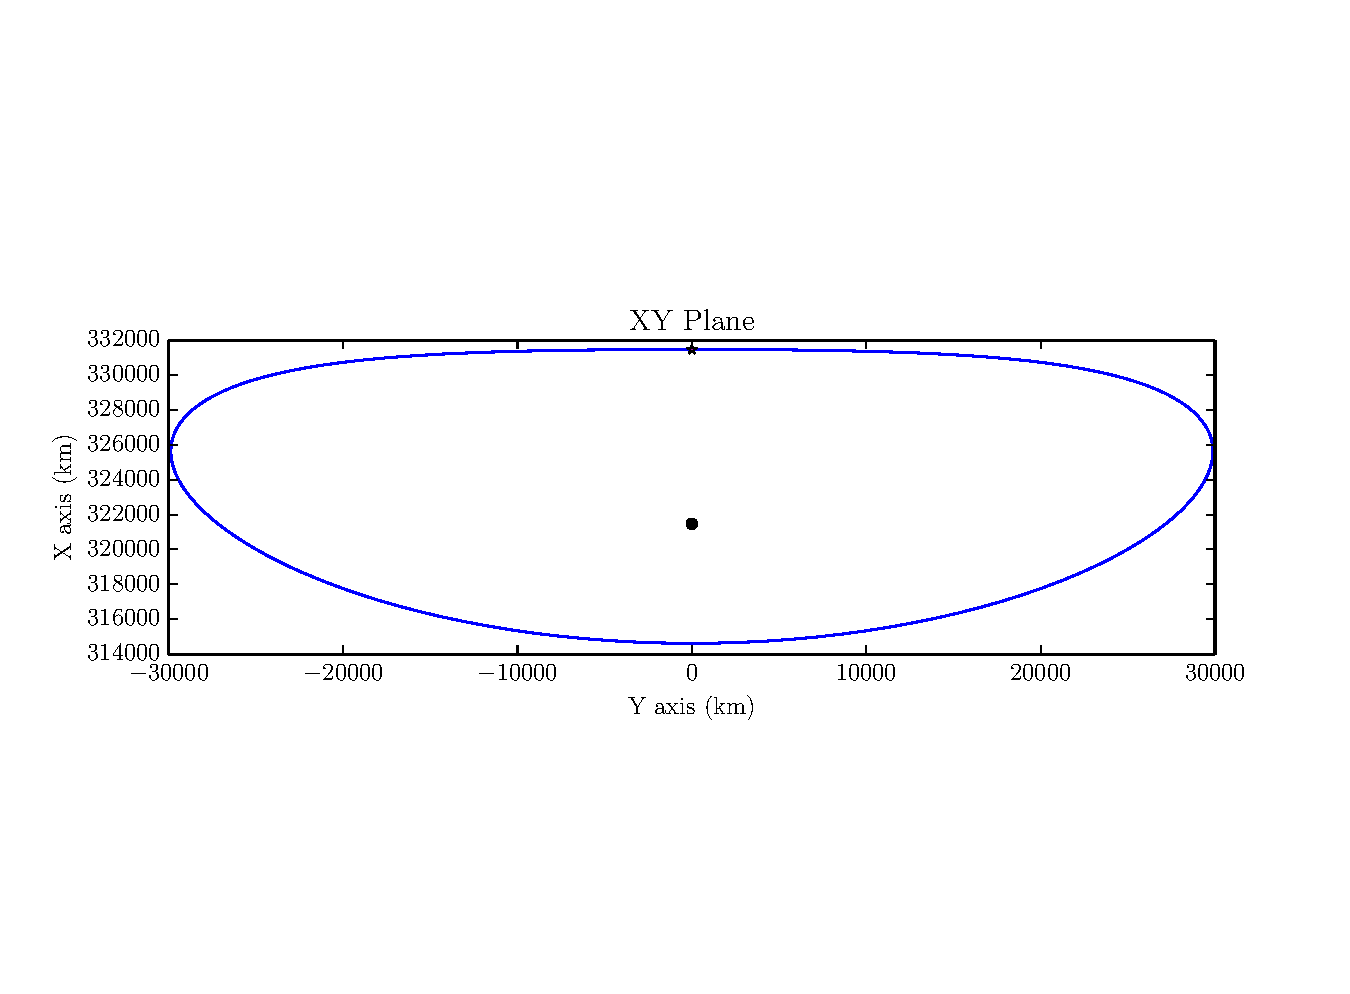
\includegraphics[width=0.9\textwidth]{Target_Full_Orbit_1}
		\caption{Target Satellite Orbit in Earth-Moon L1 CRTBP Frame}
		\label{fig:FullOrbit_1}
	\end{center}
\end{figure}

To convert between canonical and dimensional units, the relevant properties of the Earth-Moon CRTBP system are presented in Table~\ref{tab:Environment_1}.   

\begin{table}[htbp] 
	\fontsize{10}{10}\selectfont
	\caption{Earth-Moon CRTBP Parameters}
	\label{tab:Environment_1}
	\centering
	\begin{tabular}{l l}
		\hline
		Parameter   & Value \\
		\hline
		Earth mass (kg) & 5.97219e24 \\
		Moon mass (kg) & 7.34767309e22 \\
		Mass ratio \(\mu\)      & 0.012277471 \\
		Combined mass (kg), or 1 MU & 6.045667e24 \\
		\(r_{12}\) (km), or 1 DU & 384400.0 \\
		Time Constant (s), or 1 TU & 375201.9 \\
		Period of Moon around Earth (s) & 2\(\pi\)TU \\
		\hline
	\end{tabular}
\end{table}

Three waypoints are defined for the chaser satellite to travel between on its rendezvous with the target, with a final waypoint located at the target satellite itself.  The waypoint locations are presented in Table~\ref{tab:Waypoints_1} in the RIC reference frame.  The waypoints are converted into the CRTBP frame for the propagation.  Note that these waypoints represent an approach along the \(\mathbf{I}\) axis of the RIC frame. 

\begin{table}[htbp] 
	\fontsize{10}{10}\selectfont
	\caption{Waypoints in RIC Frame}
	\label{tab:Waypoints_1}
	\centering
	\begin{tabular}{ccccc}
		\hline
		Waypoint   & Time (days) & R (km) & I (km) & C (km) \\
		\hline
		1 & 0.00 & 0.0 & 15.0 & 0.0 \\
		2 & 0.36 & 0.0 & 5.0 & 0.0 \\
		3 & 0.97 & 0.0 & 1.0 & 0.0 \\
		4 & 1.59 & 0.0 & 0.0 & 0.0 \\
		\hline
	\end{tabular}
\end{table} 

Figure~\ref{fig:RIC_1} shows the result of propagating the target and chaser satellite through a rendezvous using these waypoints.  The integration is performed in the CRTBP frame, and the results are converted to the RIC frame for visualization, with the target satellite at the origin and the chaser satellite offset with respect to the target shown in kilometers.  The green curve shows the path of the chaser satellite when propagated using the linear relative motion dynamics as given in Equation~\eqref{eq:RelmoDerivs}, with the application of impulsive \(\Delta V\)'s as computed using Equation~\eqref{eq:RequiredVelocity}.  The model employed to compute the impulsive maneuvers matches the linear propagation model, and so the chaser satellite travels precisely to each waypoint.  The red curve shows the result when the chaser satellite is propagated using the nonlinear CRTBP dynamics as shown in Equation~\eqref{eq:CRTBP} when the nominal \(\Delta V\)s (as computed using the linear model) are still applied.  It is easily seen that the nominally planned maneuvers do not bring the chaser exactly to the desired waypoints when propagating with the nonlinear model. In this test, the trajectory is then reset to start at the correct waypoint in order to visualize the trajectory for the next segment. Finally, the blue curve shows the result when the chaser satellite is propagated using the nonlinear CRTBP dynamics and the \(\Delta V\)s have been corrected (or ``targeted") through the iterative differential correction procedure described above.  The path does not precisely match the original green curve due to the different dynamical models in use; however, each waypoint is achieved successfully.  % TODO: (Also note that the image axes are not scaled equally.)

\begin{figure}[htb] 
	\begin{center}
		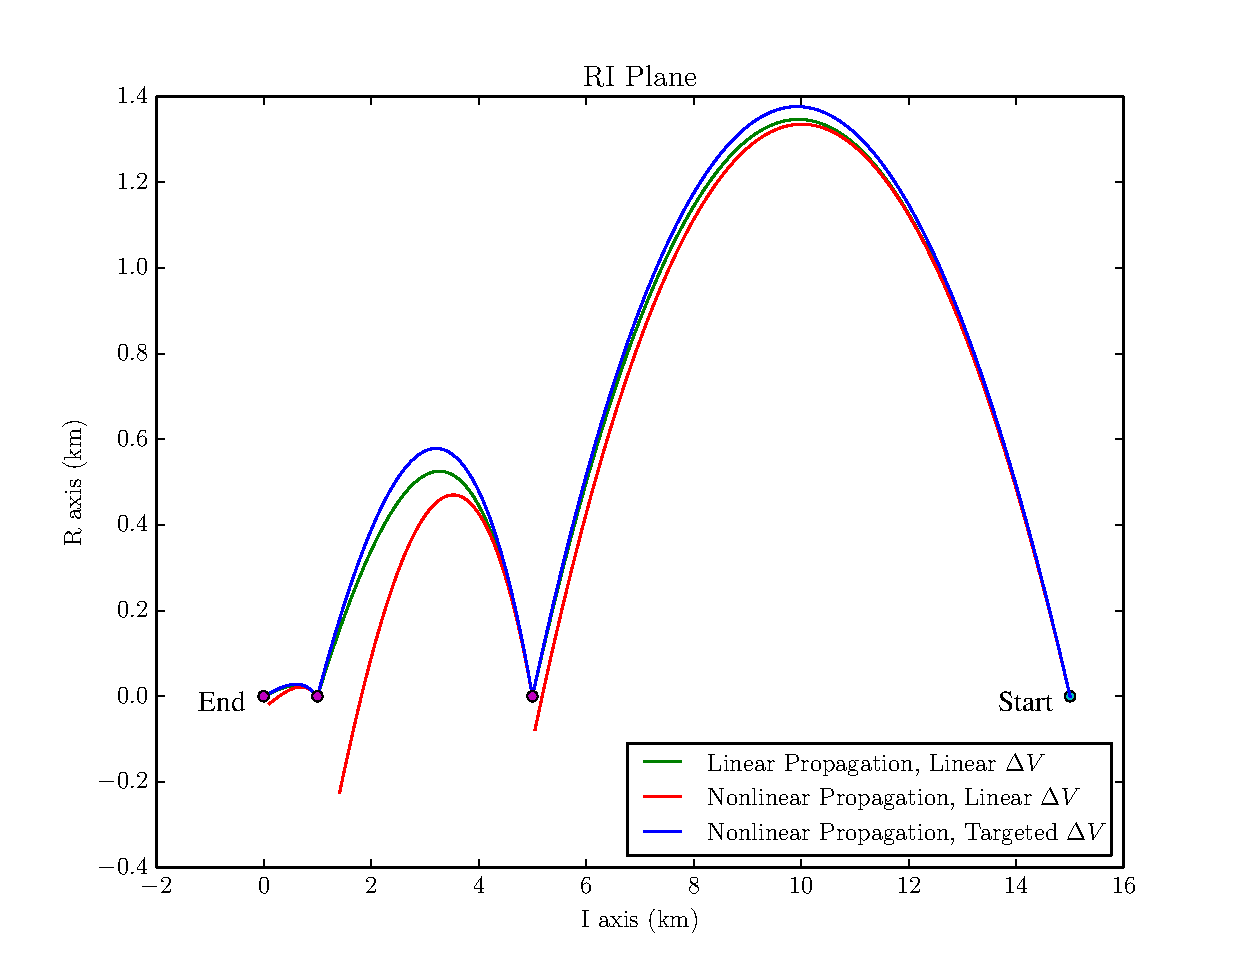
\includegraphics[width=0.9\textwidth]{RIC_1}
		\caption{Relative Motion of a Chaser Satellite with respect to a Target}
		\label{fig:RIC_1}
	\end{center}
\end{figure} % TODO: add more context/description to the captions for the plots

The results for this case are also summarized in Table~\ref{tab:Results_1}.  To compute the first \(\Delta V\), the chaser satellite is assumed to start precisely at waypoint 1 with its pre-maneuver velocity at waypoint 1 equal to the target satellite's initial velocity in the CRTBP frame.  The final maneuver at waypoint 4 is computed to equalize the chaser's velocity with the target satellite's velocity for a completed rendezvous.

We can note that, while the difference in \(\Delta V\) magnitude is quite small between the linear computation and the differentially corrected computation, on the order of millimeters/second, the angular difference between the two \(\Delta V\) vectors is more significant, reaching almost 6\textdegree \- at waypoint 3.  These differences result in achieved position errors on the order of hundreds of meters at each waypoint when the linear approximation is applied in the nonlinear propagation model; the errors are reduced to the order of centimeters when the differential correction procedure is applied.

Regarding the tuning parameters of the differential correction procedure, the perturbation value for the velocity components was set to 1e-5 DU/TU (or speed units, SU), which equals about 1.0 centimeters/second.  The tolerance on the achieved waypoints was set to 1e-9 DU, or about 0.38 meters.  

% Python Configuration for these results:
% halo_cases = ['EM']
% clock_angles = np.array([0.0])
%approach_cases = ['+R', '-R', '+I', '-I', '+C', '-C']
%timescales = ['fast', 'medium', 'slow']
%spacings = ['close', 'medium', 'far']
% not used at this time: timescales, spacings
%halo = halo_cases[0]
%clock_angle = clock_angles[0]
% approach = '+I'
%timescale = timescales[0]
%spacing = spacings[0]

% TODO: say this, maybe: The maximum number of allowed iterations was set to 10, meaning that if the desired tolerance is not achieved within 10 iterations, the process will continue with the value achieved by the \(10^{th}\) iteration.  

% TODO: discuss how many iterations were actually used.  

% TODO: add this comment: (Note that we use the *new* achieved waypoint to re-compute the linear dV estimate for the next waypoint before then targeting the next waypoint)

\begin{table}[htbp] 
	\fontsize{10}{10}\selectfont
	\caption{\(\Delta\)V and Position Error Summary at each Waypoint}
	\label{tab:Results_1}
	\centering
	\begin{tabular}{c p{0.8 cm} p{1.2 cm} p{1 cm} p{1 cm} p{1.3cm} p{1.3cm}}
		\hline
		Waypoint   & Linear \(\Delta V\) & Corrected \(\Delta V\) & \(\Delta V\)  \mbox{Angle} Difference & \(\|\Delta V \|\) Difference & Position \mbox{Error}, Linear \(\Delta V\) & Position \mbox{Error}, \mbox{Corrected} \(\Delta V\) \\
		& (m/s) & (m/s) & (deg) & (m/s) & (m) & (m) \\
		\hline
		1 & 0.346 &	0.345 &	0.466 &	-0.001 &	N/A &	N/A \\
		2 & 0.293 &	0.295 &	2.609 &   0.002 &	91.394 &	0.011 \\
		3 & 0.064 &	0.059 &	5.890 &	-0.005 &	470.653 &	0.063 \\
		4 & 0.019 &	0.018 &	0.445 &	-0.001 &	107.663 &	0.056 \\
		Total & 0.722  & 0.717 & 9.410 & 0.008 & 669.709 & 0.131 \\
		\hline
	\end{tabular}
\end{table}

% \afterpage{\clearpage}  %TODO: remove this line and others like this

\subsection{Rendezvous Initial Clock Angle}

This technique can be used to evaluate the relative \(\Delta V\) cost of performing a rendezvous at different points along a target spacecraft's orbit.  The following orbital plots present twelve test cases that each begin with the target satellite at a different ``clock angle" in its orbit; each test case is separated by one twelfth of an orbit in time, with the twelve starting positions indicated by the asterisks shown in Figure~\ref{fig:FullOrbit_2}.

\begin{figure}[htb] 
	\begin{center}
		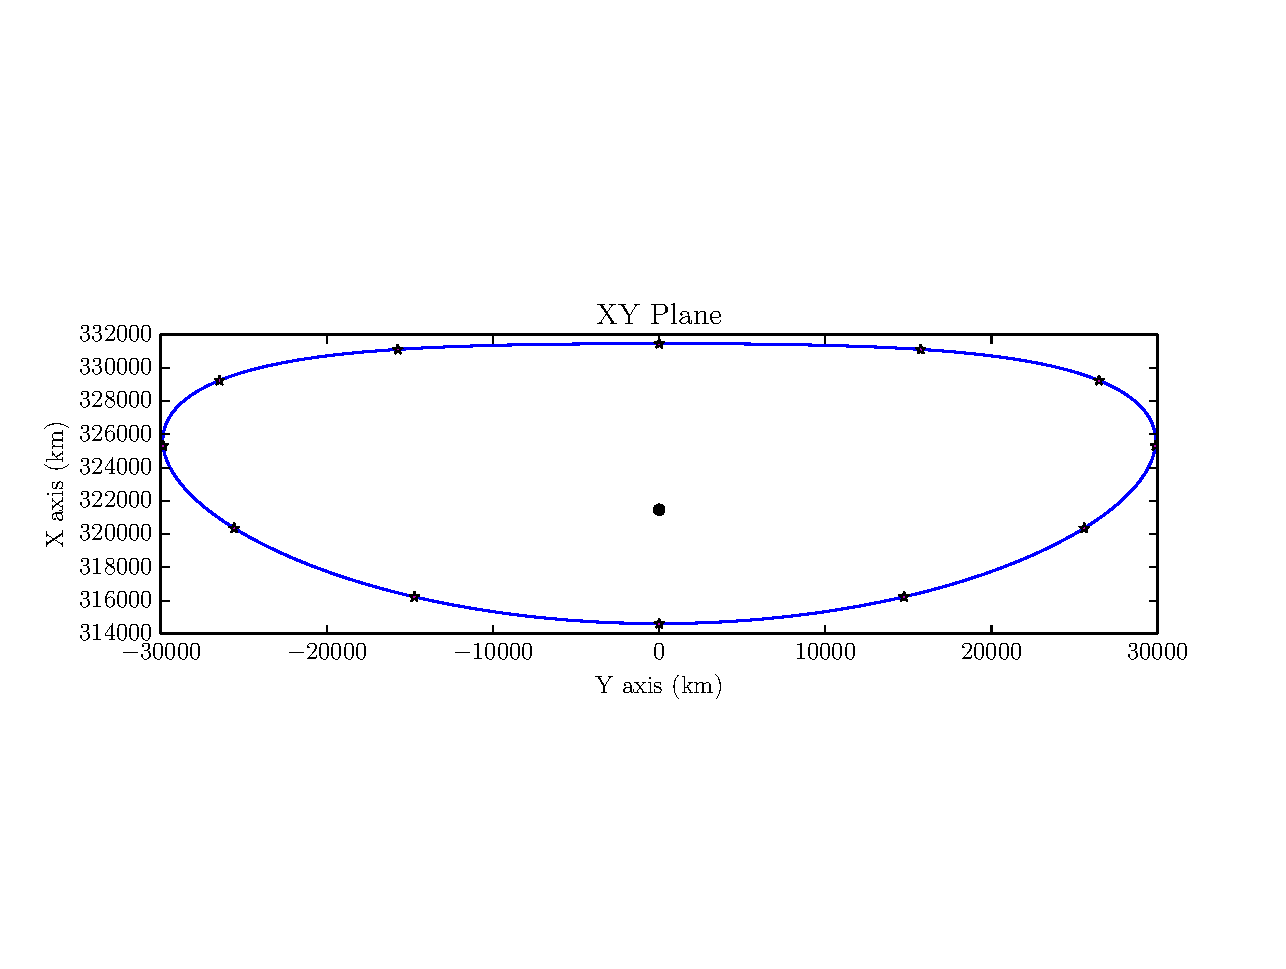
\includegraphics[width=0.8\textwidth]{Target_Full_Orbit_2}
		\caption{Twelve Target Satellite Initial Conditions}
		\label{fig:FullOrbit_2}
	\end{center}
\end{figure}

Each of these twelve rendezvous sequences are computed using the same waypoint locations along the \(\mathbf{I}\) axis of the RIC frame as shown in Table~\ref{tab:Waypoints_1}.  However, due to the differing local curvature of the target orbit at each of the twelve starting locations, the relative motion patterns in the RIC frame for each rendezvous are different, as shown in Figure~\ref{fig:RIC_2}.  

\begin{figure}[htb] 
	\begin{center}
		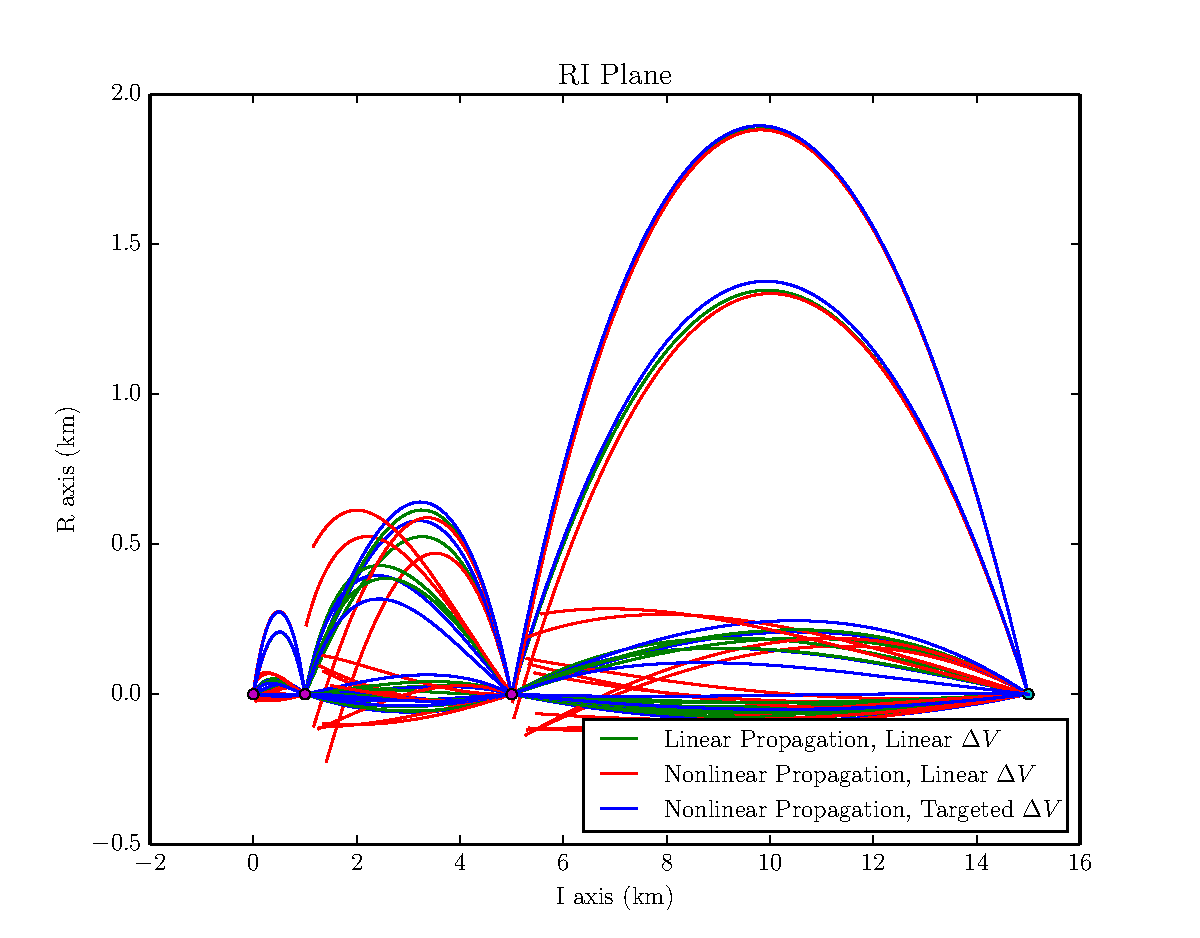
\includegraphics[width=0.8\textwidth]{RIC_2}
		\caption{Rendezvous using 12 Different Initial Clock Angles}
		\label{fig:RIC_2}
	\end{center}
\end{figure}

\clearpage

When viewed using the CRTBP reference frame's rotating axes as in Figure~\ref{fig:RLP_2}, it is more intuitively seen that each of these in-track rendezvous sequences approach the target satellite from a different direction in the CRTBP frame, due to the rotation of the RIC frame with the target satellite's orbit.

\begin{figure}[htb] 
	\begin{center}
		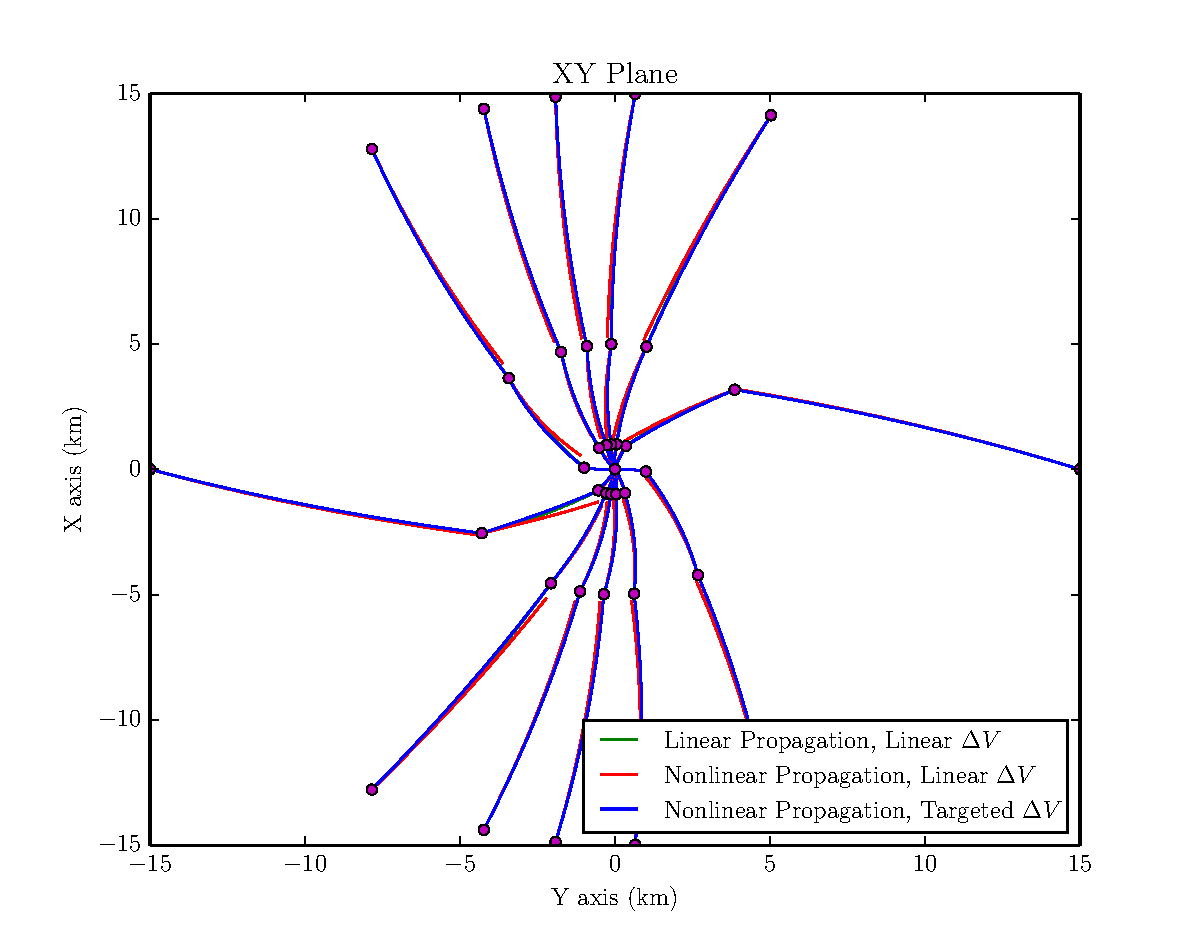
\includegraphics[width=0.9\textwidth]{RLP_2} % scale=0.5
		\caption{Rendezvous using 12 Different Initial Clock Angles; CRTBP Axes}
		\label{fig:RLP_2}
	\end{center}
\end{figure}

The same rendezvous was then computed for 360 test cases with the initial conditions spaced evenly in time around the same libration point orbit, in order to examine the trends in total \(\Delta V\) to complete the rendezvous as a function of the initial clock angle. The total \(\Delta V\) is shown in Figure~\ref{fig:DV_2} as a function of the initial clock angle; the magnitude of both the linear approximated \(\Delta V\) and the nonlinear corrected \(\Delta V\) are shown.  From this we can see that the total \(\Delta V\) cost does not change dramatically when the initial clock angle is varied; however the peak costs are at initial clock angles of 0\textdegree and 180\textdegree.  This trend is apparent in the linear approximation of the \(\Delta V\) as well as in the corrected or ``targeted" results; this means that the linear approximation may safely be used in this case to provide order-of-magnitude indications of the relative costs of the different rendezvous sequences.

\begin{figure}[htb] 
	\begin{center}
		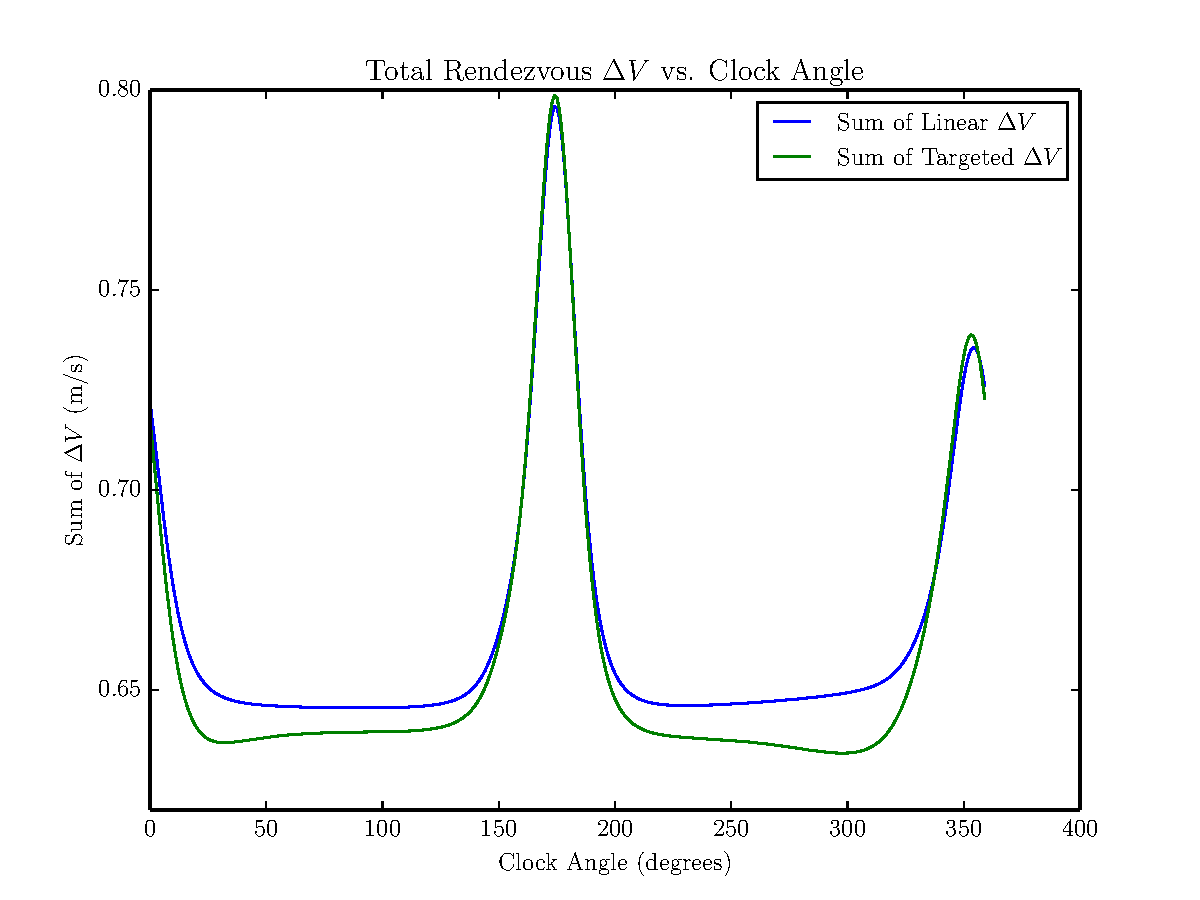
\includegraphics[width=0.9\textwidth]{Total_DV_2_1degsteps} 
		\caption{Total Rendezvous \(\Delta\)V for Different Initial Clock Angles}
		\label{fig:DV_2}
	\end{center}
\end{figure}

The total rendezvous position error, summed up over waypoints 2 through 4, is shown in Figure~\ref{fig:PosErr_2} as a function of the initial clock angle.  The position error when the linear approximated \(\Delta V\) is applied in the nonlinear model is on the order of 1e3 m, while the order of magnitude of the position error after the differential correction has been applied is 1e-1 m, which was the tolerance level of the correction algorithm and could even be improved with more differential correction iterations.

\begin{figure}[htb] 
	\begin{center}
		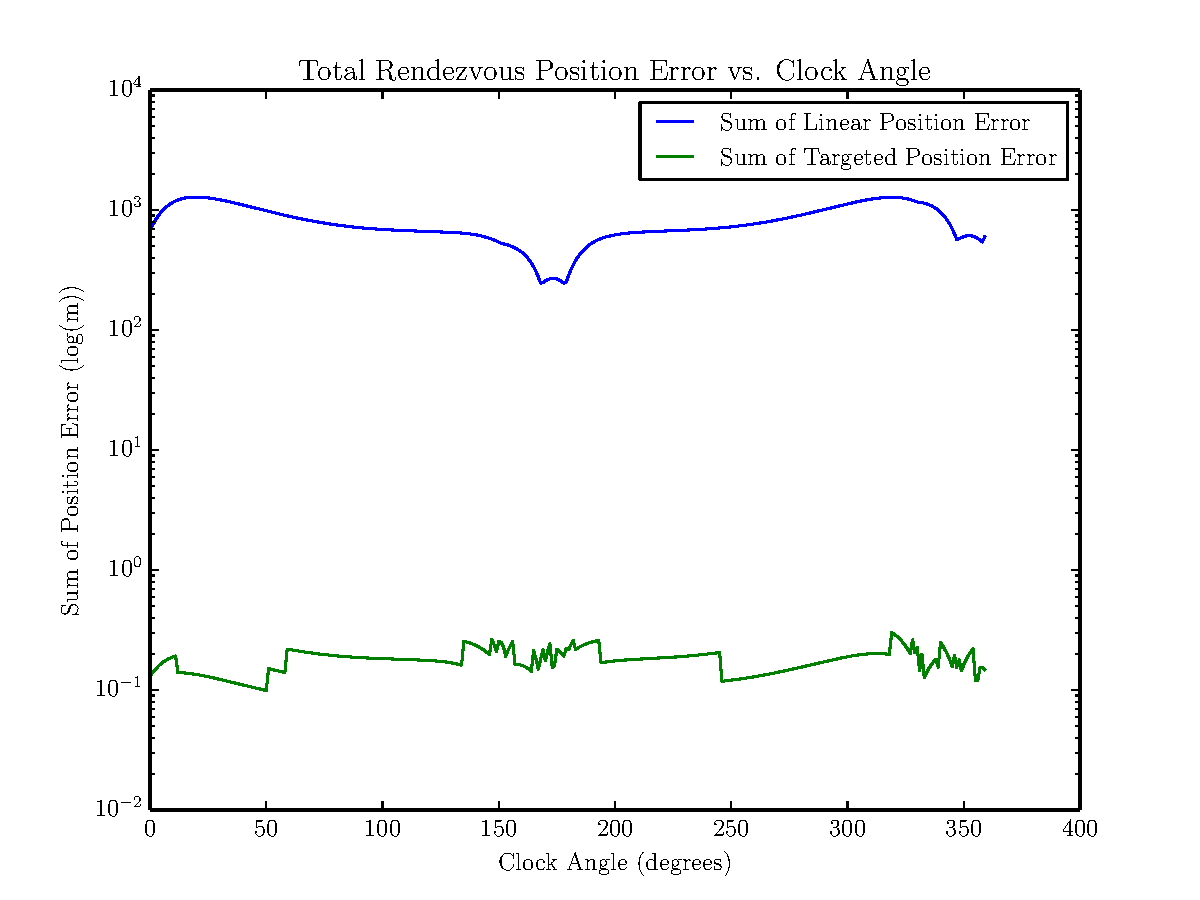
\includegraphics[width=0.8\textwidth]{Log_Position_Error_2_1degsteps} 
		\caption{Total Rendezvous Position Error for Different Initial Clock Angles}
		\label{fig:PosErr_2}
	\end{center}
\end{figure}

Although the differences in the magnitude of the \(\Delta V\) vector are not large when comparing the linear approximation to the nonlinear differential correction, the direction of the \(\Delta V\) vector is sometimes quite different. The angle between the \(\Delta V\) vectors, summed up over each impulse of the rendezvous, is shown in Figure~\ref{fig:DVAngle_2}.

\begin{figure}[htb] 
	\begin{center}
		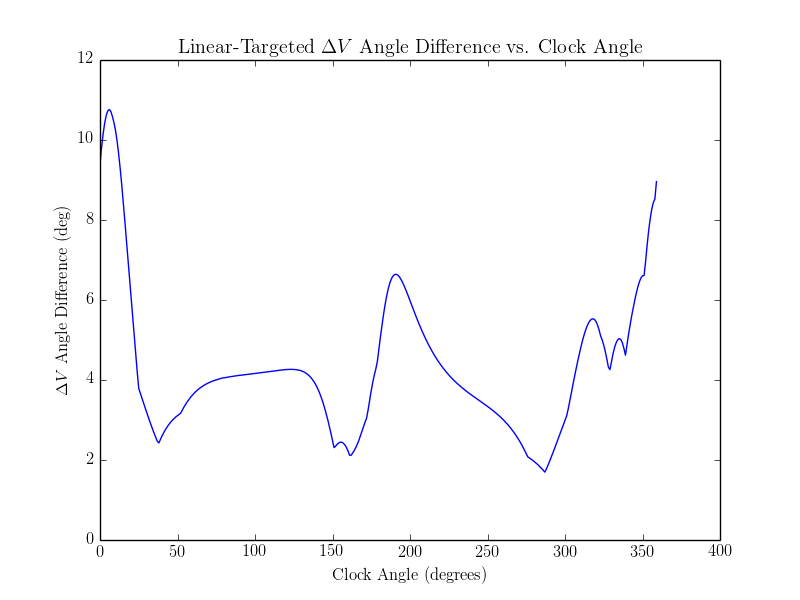
\includegraphics[width=0.8\textwidth]{DV_Angle_Diff_2_1degsteps} 
		\caption{Total Rendezvous \(\Delta\)V Angle Difference for Different Initial Clock Angles}
		\label{fig:DVAngle_2}
	\end{center}
\end{figure}

These same techniques and metrics can be used to evaluate other rendezvous approach strategies, such as approaching the target satellite with different waypoint spacing, or from a different direction, or in a different target orbit.

%TODO: conclusions section here

\clearpage

% Python Configuration for these results:
%halo_cases = ['EM']
%clock_angles = np.arange(0.0, 360.0, 30.0)  or np.arange(0.0, 360.0, 1.0), etc
%halo = halo_cases[0]
%clock_angle = clock_angles[0]
%approach = '+I'
%timescale = timescales[0]
%spacing = spacings[0]

% More TODO's:

% Show cases where we approach from different directions (+/-R, +/-I, +/-C)

% Evaluate relative cost of approaching in different ways

% From ASC abstract: The robustness of the procedure, with respect to the convergence of the differential corrector using the initial guess from the linear model, also depends on properties of the rendezvous such as the time allowed and distance traveled between waypoints.

% Distance (maybe percentage of orbit covered?) where this technique doesn't work

% Seems like shorter times maybe gives better behavior of the linear dV estimate?  Longer time = more need to use the targeter?

% What if naive initial guess was supplied?  would that require more iterations?

% Show what happens if you miss a maneuver

% Show what happens if you don't reset the linear approximated dV path back to the next waypoint

% Kinda interesting to show in RLP, VNB

% Maybe talk about measuring the "excursion" of the trajectory (perpendicular to the vector from one waypoint to the next)

%\section{Conclusions}


\section{Acknowledgment}
Any acknowledgments by the author may appear here. The acknowledgments section is optional.


\bibliographystyle{AAS_publication}   % Number the references.
\bibliography{references_Case}   % Use references.bib to resolve the labels.

\end{document}
